\documentclass[17pt,a4paper,landscape]{extarticle}
\usepackage[margin=2.35cm,top=0.12cm,left=1.05cm]{geometry}
\usepackage{amsmath}
\usepackage{amssymb}
\usepackage{tasks}
\usepackage{tikz}
\usepackage{xcolor}
\usepackage[sfdefault,lf]{FiraSans}
\renewcommand{\familydefault}{\sfdefault}
\setlength{\parindent}{0pt}
\pagestyle{empty}
\settasks{label=\textbf{\arabic*.}, label-width=2.2em, item-indent=2.95em, column-sep=2.1cm, after-item-skip=4.7em}
\renewcommand{\arraystretch}{1.15}
\everymath{\displaystyle}

\begin{document}
\sffamily
\boldmath

\boldmath

\boldmath

{\LARGE \textbf{Angles on a straight line --- Proficient}}
\begin{tasks}(3)
\task {Find \mbox{$x$}.\\[0.4em]
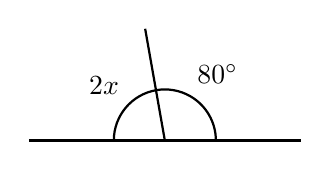
\begin{tikzpicture}[scale=0.72,baseline=(current bounding box.center)]
\draw[thick] (-2.4,0)--(0,0)--(2.4,0);
\draw[thick] (0,0)--({2*cos(100)},{2*sin(100)});
\draw[thick] (0.9,0) arc[start angle=0,end angle=100,radius=0.9];
\draw[thick] ({0.9*cos(100)},{0.9*sin(100)}) arc[start angle=100,end angle=180,radius=0.9];
\node at ({1.45*cos(50)},{1.45*sin(50)+0.06}) {$80^\circ$};
\node at ({1.4*cos(140)},{1.4*sin(140)+0.06}) {$2x$};
\end{tikzpicture}}
\task {Find \mbox{$y$}.\\[0.4em]
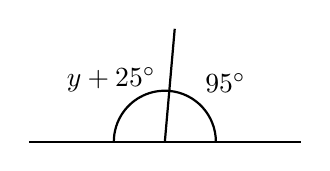
\begin{tikzpicture}[scale=0.72,baseline=(current bounding box.center)]
\draw[thick] (-2.4,0)--(0,0)--(2.4,0);
\draw[thick] (0,0)--({2*cos(85)},{2*sin(85)});
\draw[thick] (0.9,0) arc[start angle=0,end angle=85,radius=0.9];
\draw[thick] ({0.9*cos(85)},{0.9*sin(85)}) arc[start angle=85,end angle=180,radius=0.9];
\node at ({1.45*cos(42.5)},{1.45*sin(42.5)+0.06}) {$95^\circ$};
\node at ({1.4*cos(132.5)},{1.4*sin(132.5)+0.06}) {$y+25^\circ$};
\end{tikzpicture}}
\task {Find \mbox{$a$}.\\[0.4em]
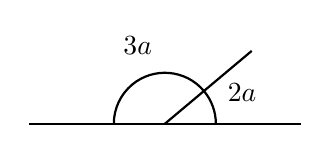
\begin{tikzpicture}[scale=0.72,baseline=(current bounding box.center)]
\draw[thick] (-2.4,0)--(0,0)--(2.4,0);
\draw[thick] (0,0)--({2*cos(40)},{2*sin(40)});
\draw[thick] (0.9,0) arc[start angle=0,end angle=40,radius=0.9];
\draw[thick] ({0.9*cos(40)},{0.9*sin(40)}) arc[start angle=40,end angle=180,radius=0.9];
\node at ({1.45*cos(20)},{1.45*sin(20)+0.06}) {$2a$};
\node at ({1.4*cos(110)},{1.4*sin(110)+0.06}) {$3a$};
\end{tikzpicture}}
\task {Find \mbox{$b$}.\\[0.4em]
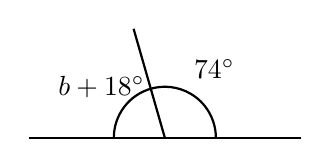
\begin{tikzpicture}[scale=0.72,baseline=(current bounding box.center)]
\draw[thick] (-2.4,0)--(0,0)--(2.4,0);
\draw[thick] (0,0)--({2*cos(106)},{2*sin(106)});
\draw[thick] (0.9,0) arc[start angle=0,end angle=106,radius=0.9];
\draw[thick] ({0.9*cos(106)},{0.9*sin(106)}) arc[start angle=106,end angle=180,radius=0.9];
\node at ({1.45*cos(53)},{1.45*sin(53)+0.06}) {$74^\circ$};
\node at ({1.4*cos(143)},{1.4*sin(143)+0.06}) {$b+18^\circ$};
\end{tikzpicture}}
\task {Find \mbox{$c$}.\\[0.4em]
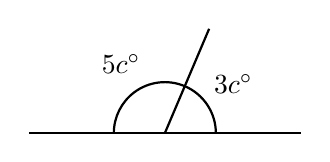
\begin{tikzpicture}[scale=0.72,baseline=(current bounding box.center)]
\draw[thick] (-2.4,0)--(0,0)--(2.4,0);
\draw[thick] (0,0)--({2*cos(67)},{2*sin(67)});
\draw[thick] (0.9,0) arc[start angle=0,end angle=67,radius=0.9];
\draw[thick] ({0.9*cos(67)},{0.9*sin(67)}) arc[start angle=67,end angle=180,radius=0.9];
\node at ({1.45*cos(33.5)},{1.45*sin(33.5)+0.06}) {$3c^\circ$};
\node at ({1.4*cos(123.5)},{1.4*sin(123.5)+0.06}) {$5c^\circ$};
\end{tikzpicture}}
\task {Find \mbox{$d$}.\\[0.4em]
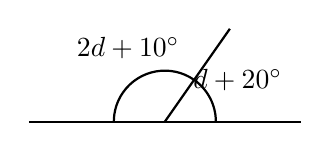
\begin{tikzpicture}[scale=0.72,baseline=(current bounding box.center)]
\draw[thick] (-2.4,0)--(0,0)--(2.4,0);
\draw[thick] (0,0)--({2*cos(55)},{2*sin(55)});
\draw[thick] (0.9,0) arc[start angle=0,end angle=55,radius=0.9];
\draw[thick] ({0.9*cos(55)},{0.9*sin(55)}) arc[start angle=55,end angle=180,radius=0.9];
\node at ({1.45*cos(27.5)},{1.45*sin(27.5)+0.06}) {$d+20^\circ$};
\node at ({1.4*cos(117.5)},{1.4*sin(117.5)+0.06}) {$2d+10^\circ$};
\end{tikzpicture}}
\task {The angle next to \mbox{$4x^\circ$} on a straight line is \mbox{$(x+30)^\circ$}. Find \mbox{$x$}.}
\task {The angle next to \mbox{$(2m+10)^\circ$} on a straight line is \mbox{$(m+50)^\circ$}. Find \mbox{$m$}.}
\task {Two adjacent angles on a straight line are equal. What is each angle?}
\task {One angle on a straight line is three times the other. Find both angles.}
\task {One angle on a straight line is \mbox{$26^\circ$} bigger than the other. Find both angles.}
\task {Explain how you know that \mbox{$112^\circ$} and \mbox{$68^\circ$} could be adjacent angles on a straight line.}
\end{tasks}

\end{document}
